\chapter{Background Theory}
The intended outcome of this literature review is to deliver a thorough explanation of the various technologies used throughout the project and to provide detail on any additional subject matter aspects which will aid understanding of the project. 

A general summation of Big Data and its application is given in section \ref{bigdata} which is followed by a discussion on the pre-processing of datasets discussed in section \ref{etl}. A high level overview of the NoSQL concept is examined in section \ref{nosql}. The various types of dataset classification which are utilised in the project are given in section \ref{dbclass}.

The majority of the research conducted in this literature review reflects that of user manuals.

\section{Big Data}\label{bigdata}
Big Data is a broad evolving term bound to a complex and powerful application of analytical insight which over recent years has had a variety of definitions. In simplistic terms Big Data can be described as extremely large datasets that may be studied computationally to reveal patterns, trends, and associations for ongoing discovery and analysis.

\subsection{5vs Model}
In 2001, Gartner analyst Doug Laney delivered the original 3vs model which define the challenges and opportunities which have arisen by the increase in data volumes. Laney categorises big data in to three dimensions; Volume, Velocity and Variety, with the increase of each encapsulating the challenges currently faced today of big data management. The characteristics of each property are defined as \textbf{Volume} - Refers to the bast amounts of data generated every second. With the creation and storage of large quantities of data, the scale of this data becomes progressively vast. \textbf{Velocity} - Refers to the speed at which new data is generated and the speed at which data moves around emphasising the "timeliness" of the big data. In order to fully profit from the commercial value of big data, data collection and data examination must be conducted promptly . \textbf{Variety} - This characteristic alludes to the various types of data we can now use; semi-structured and unstructured. Examples being "audio, video, webpage and text as well as traditional structured data" (Chen, Mao, Zhang and CMeung REF).

The amount of data being produced has dramatically increased from when Laney first brought us the 3vs model in 2001. Big Data is a term becoming more and more common in business and society. Overcoming obstacles and implementing effective, actionable Big Data strategies is key for successful big data management. IBM has introduced a fourth V, Veracity \textbf{Veracity} Data inconsistencies and incompleteness result in data uncertainty and unreliability. This creates a new challenge; keeping data organised. (Big Data ref)

The final and considered by many to be the most important V of big data is \textbf{Value}. "All the volumes of fast-moving data of different variety and veracity have to be turned into value" (IBM ref) One of the biggest challenges faced by organisations is having the ability to turn data into value. \textbf{Value} Refers to ones ability to turn big data into something useful and which adds value to your organisation.

\section{Extract Transform Load}\label{etl}
A basic definition of the Extract Transform Load (ETL) process is pulling data out of one database, refactoring the composition of the data and putting the data into another database. - EXPAND

\subsection{Process}
ETL is a three step procedure which combines database functions into one tool. - EXPAND

\subsubsection{Extract} is the first step in the ETL procedure in which data is read from a database. The Extract step covers the data extraction from the source system and makes it accessible for further processing. The main objective of the extract step is to retrieve all the required data from the source system with as little resources as possible. The extract step should be designed in a way that it does not negatively affect the source system in terms or performance, response time or any kind of locking.

\subsubsection{Transform} where the extracted data is manipulated from its previous state and converted into another database format. The transform step applies a set of rules to transform the data from the source to the target. This includes converting any measured data to the same dimension (i.e. conformed dimension) using the same units so that they can later be joined. The transformation step also requires joining data from several sources, generating aggregates, generating surrogate keys, sorting, deriving new calculated values, and applying advanced validation rules.

\subsubsection{Load} completes the three step procedure and is where data is written into the target database. During the load step, it is necessary to ensure that the load is performed correctly and with as little resources as possible. The target of the Load process is often a database. In order to make the load process efficient, it is helpful to disable any constraints and indexes before the load and enable them back only after the load completes. The referential integrity needs to be maintained by ETL tool to ensure consistency.

\subsection{Tool Implementation}


Apache Jena (Jena) is a free and open source Java framework for building semantic web and Linked Data applications. (JENA REF) The Jena framework  of different APIs interacting together to process RDF data.

\section{Knowledge Representation Languages}
A Knowledge Representation (KR) language can be defined as for any given interpretation of a sentence or string of text the KR must have the ability to effectively and unambiguously express knowledge in a both a human and computer manageable form. 

There are a number of options and possibilities for communicating data and information which range from binary representation to meta markup languages such as Extensible Markup Language (XML) for example. Markup languages which are easily read by humans such as XML which as a result of its rigid set of rules lends its self to both humans and machines. Comparatively binary notation which uses 1's and 0's to represent data, while relatively cheap in terms of computing power the ability to comprehend this notation requires a unique and specific skill set.

\subsection{Semantic Web}
The Semantic Web is an extension of the Web through standards by the World Wide Web Consortium (W3C). The standards promote common data formats and exchange protocols on the Web, most fundamentally the Resource Description Framework (RDF).

The Semantic Web is about two things. It is about common formats for integration and combination of data drawn from diverse sources, where on the original Web mainly concentrated on the interchange of documents. It is also about language for recording how the data relates to real world objects. That allows a person, or a machine, to start off in one database, and then move through an unending set of databases which are connected not by wires but by being about the same thing.

\subsection{Web Ontology Language OWL}\label{owl}
The Web Ontology Language OWL is a language representation standard for designing and authoring Web ontologies produced from the World Wide Web Consortium W3C. (OWL REF). The OWL file format is designed to be used by applications required to process the content of the information and to be humanly readable. "[OWL] is intended to provide a language that can be used to describe the classes and relations between them that are inherent in Web documents and applications." (OWL REF). 

The OWL languages are characterised by formal semantics. They are built upon a W3C XML standard for objects called the Resource Description Framework (RDF).

\subsection{OBO}\label{obo}
The OBO flat file format is an ontology representation language (OBO ref) The OBO flat file format is an ontology representation language. The concepts it models represent a subset of the concepts in the OWL description logic language, with several extensions for meta-data modelling and the modelling of concepts that are not supported in DL languages.

The format itself attempts to achieve the following goals:

Human readability
Ease of parsing
Extensibility
Minimal redundancy


\section{NoSQL}\label{nosql}
NoSQL is labeled as a next generation database known to most as "Not only SQL" (NOSQL REF). This definition however insinuates its defiance against the once industry standard SQL. It was originally developed in 1998 by Carlo Strozzi; a member of the Italian Linux society, with the intention of being a non-relational, widely distributable and highly scalable database. Strozzi named the database management system NoSQL to merely state it does not express queries in the traditional SQL format. Sadalage and Fowler believe the definition we commonly refer NoSQL as comes from a 2009 conference in San Fransisco held by Johan Oskarsson, a software developer. Sadalage and Fowler recall Oskarssons desire to generate publicity surrounding the event and in an attempt to do so devised the twitter hashtag "NoSQL Meetup". The main attendees at the conference debrief session were Cassandra, CouchDB, HBase and MongoDB and so the association stuck. (Sadalage and Fowler ref)

There are are number of key features which encompass the NoSQL framework and encapsulate the essence of its popularity. Many of the NoSQL databases boast their capacity of working in a cluster environment - a cluster being two or more connected computers working collaboratively. Thus delivering a range of options for consistency and distribution (Sadalage and Fowler ref) (Section \ref{distributeddb}).

NoSQL solutions are not bound by a definitive schema structure. This permits the ability to freely adapt database records or add custom fields for example without considering structural changes. This is extremely effective when dealing with varying data types and data sets, in comparison to the traditional relational database model which when tackling this issue often resulted in ambiguous field names. (Sadalage and Fowler ref)

\section{Database Classification}\label{dbclass}
One of the first decisions to be made when when selecting a database is the characteristics of the data you are looking to leverage. (Dash, 2013) There are a multitude of options available with many different classifications. - \textcolor{red}{EXPAND}

\subsection{Distributed Database}\label{distributeddb}
A distributed database (DDB) comprises of two or more data files located at different sites and servers on a computer network. (DD ref) The advantage of using a DD is that as the database is distributed, multiple users can access a portion of the database at different locations locally and remotely without obstructing one another's work. It is  pivotal for the DD database management system to periodically synchronise the scattered databases to make sure that they all have consistent data. (DD ref) For example if a user updates or deletes data in one location is is essential this change is mirrored on all databases. This ability to remotely access a database from all across the world lends itself to not only multinational companies for example but also startup businesses which recruit the expertise of others from various locations.

\subsection{Document-Oriented Database}
Document-orientated database (DODB) are designed for storing, retrieving and managing document files such as XML, JSON and BSON. The documents stored in a DODB model are data objects which describe the data in the document, as well as the data itself. - EXPAND

\subsection{Graph-Orientated Database}
A graph-oriented database (GODB), is a form of NoSQL database solution that uses graph theory to store, map and query relationships. A graph is a collection of nodes connected by relationships. "Graphs represent entities as nodes and the ways in which those entities relate to the world as relationships." (Robinson, Webber and Eifrem, 2015) The formation of the graph database structure is extremely useful and eloquent as it permits clear modelling of a vast and often ecliptic array of data types. (Robinson, Webber and Eifrem, 2015) An example of data represented in a graph structure is the Twitter relationship model. \begin{center}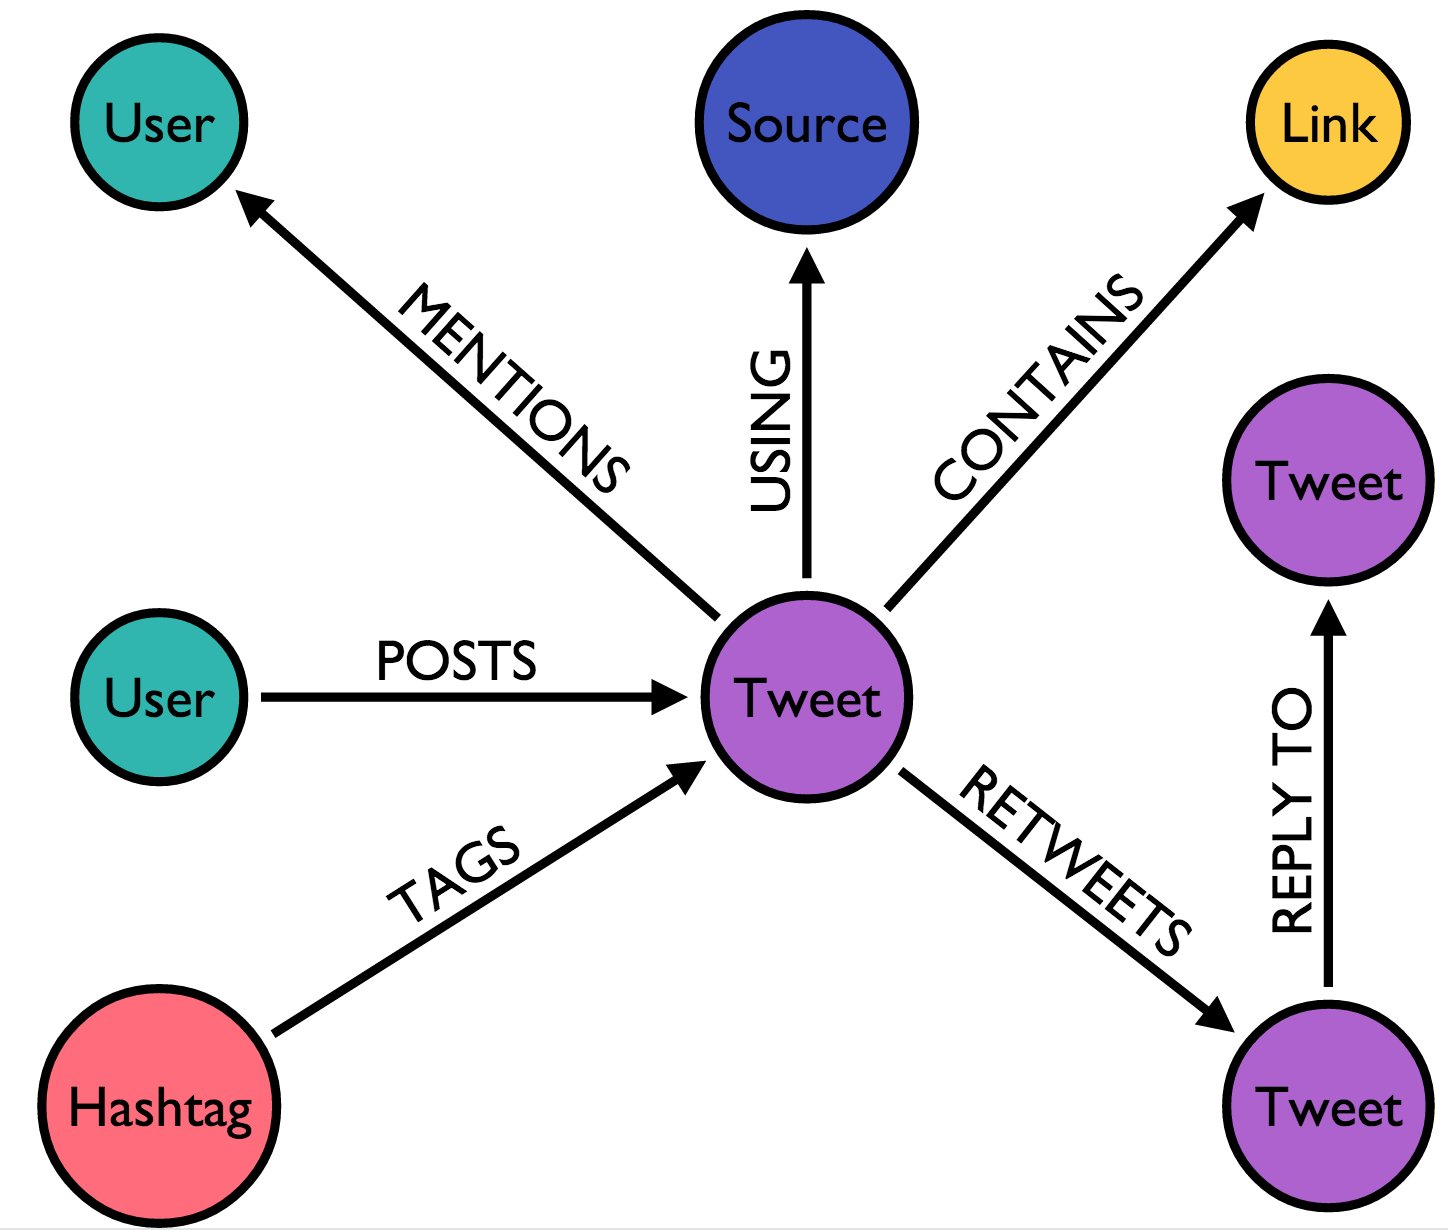
\includegraphics[width=0.5\linewidth]{images/graphdb_twitter}\end{center}  Figure[ADD FIGURE REF] illustrates the nodes involved in a standard tweet and the relationship link between them. The labeled nodes indicate the various operations which are involved in one the tweet. One interpretation of the [FIGURE REF] example is that a user posts a tweet, using the Twitter App which mentions another user and includes a hashtag and link. - \textcolor{red}{REVISE}

\subsection{Relational Database}
A relational database (RDB) is a collection of data items organised as a set of tables, records and columns from which data can be accessed or reassembled in many different ways. (RDB ref)  \begin{center}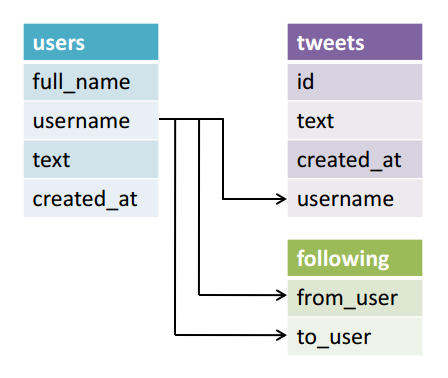
\includegraphics[width=0.75\linewidth]{images/rdbmsmodel}\end{center}The connected tables are known as relations and contain one or more columns which comprise of data records called rows. Relations can also be instantiated between the data rows to form functional dependencies called keys which are classified as : (RDB ref 2)

\begin{itemize}
\item One to One: One table record relates to another record in another table.
\item One to Many: One table record relates to many records in another table.
\item Many to One: More than one table record relates to another table record.
\item Many to Many: More than one table record relates to more than one record in another table.
\end{itemize}




